% !TEX program = xelatex
\documentclass[aspectratio=169,11pt]{beamer}

% --- Theme -------------------------------------------------------------
\usetheme{metropolis}
\metroset{progressbar=frametitle, numbering=fraction, block=fill}

% --- Packages ----------------------------------------------------------
\usepackage{graphicx}
\usepackage{amsmath,amssymb}
\usepackage{booktabs}
\usepackage{tikz}
\usetikzlibrary{arrows.meta, positioning, shapes.geometric}
\usepackage{xcolor}

% --- Figures path ------------------------------------------------------
\graphicspath{{../../outputs/figures/}}

% --- Colors (metropolis accent) ----------------------------------------
\definecolor{bluex}{HTML}{1F77B4}
\definecolor{redx}{HTML}{D62728}
\definecolor{grayx}{HTML}{555555}

% --- Metadata ----------------------------------------------------------
\title{Measuring the Universe with Sound Waves}
\subtitle{A From-Scratch Cosmology Simulation + Analysis Pipeline}
\author{Dennis Wu}
\institute{PHY\,305 \textendash{} Creative Project}
\date{April 2026}

% ======================================================================
\begin{document}

% ---------------------------------------------------------------- Title
\maketitle

% -------------------------------------------------------- 1. Motivation
\begin{frame}{The big idea: a sound wave left a ruler in the sky}
  \small
  \begin{columns}[T]
    \column{0.56\textwidth}
    \textbf{Before atoms formed} ($t < 380{,}000$ yr): the universe
    was a hot photon--baryon plasma coupled by Thomson scattering.

    \smallskip
    Overdensities launched \textbf{spherical sound waves} at
    $c_s \approx c/\sqrt{3}$. When photons decoupled, the waves
    \textbf{froze in place} at a comoving radius
    $r_s \approx 150~\mathrm{Mpc}$ --- a fixed ruler in the matter
    distribution.

    \smallskip
    Today we see it as a \textbf{bump in $\xi(r)$} near
    $100~h^{-1}$Mpc and \textbf{wiggles in $P(k)$}.

    \smallskip
    The CMB pins $r_s$ exactly, so BAO is a
    \alert{cosmic standard ruler} --- measuring its apparent size
    at any redshift gives $H(z)$, $d_A(z)$, and constraints on
    dark energy.

    \column{0.44\textwidth}
    \centering
    \includegraphics[width=\linewidth]{pk_input.png}\\
    {\scriptsize Linear $P(k)$ (top) and the wiggle ratio
      $P(k)/P_{\rm no\text{-}wiggle}(k)$ (bottom).
      Those few-percent oscillations \emph{are} BAO.}
  \end{columns}
\end{frame}

% ---------------------------------------------------- 1b. Why it's hard
\begin{frame}{Why measuring BAO is hard}
  \small
  \textbf{Problem 1 --- gravity smears the ruler.}
  Galaxies drift toward overdense regions, blurring the BAO bump
  by several $h^{-1}$Mpc. \\
  \alert{Fix: reconstruction} --- estimate where galaxies came
  from and move them back.

  \smallskip
  \textbf{Problem 2 --- the wiggles ride on a huge smooth signal.}
  Our simulation's finite resolution also distorts that smooth
  shape. \\
  \alert{Fix: broadband marginalization} --- fit the smooth shape
  as a nuisance; only the oscillations constrain the ruler.

  \smallskip
  \textbf{Problem 3 --- one universe $=$ one noisy measurement.} \\
  \alert{Fix: 100 fake ``mock'' universes} to estimate error bars
  (a covariance matrix).

  \smallskip
  \begin{center}
  \footnotesize
  This project $=$ a pipeline that simulates a piece of universe,
  measures BAO, fixes all three problems, and checks the answer.
  \end{center}
\end{frame}

% --------------------------------------------------------- 2. Pipeline
\begin{frame}{The pipeline in one picture}
  \vspace{-0.2em}
  \centering
  \scalebox{0.85}{%
  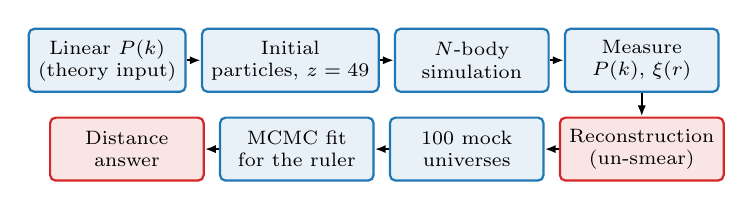
\begin{tikzpicture}[
      node distance=0.3cm and 0.18cm,
      stage/.style={rectangle, rounded corners=2pt, draw=bluex, thick,
                    fill=bluex!10, align=center, minimum height=0.8cm,
                    minimum width=1.95cm, font=\scriptsize},
      arr/.style={-{Latex[length=1.4mm]}, thick}
    ]
    \node[stage] (pk)    {Linear $P(k)$\\(theory input)};
    \node[stage, right=of pk]    (ic)    {Initial\\particles, $z=49$};
    \node[stage, right=of ic]    (nb)    {$N$-body\\simulation};
    \node[stage, right=of nb]    (est)   {Measure\\$P(k)$, $\xi(r)$};
    \node[stage, below=of est,fill=redx!12,draw=redx]  (rec)   {Reconstruction\\(un-smear)};
    \node[stage, left=of rec]    (cov)   {100 mock\\universes};
    \node[stage, left=of cov]    (mcmc)  {MCMC fit\\for the ruler};
    \node[stage, left=of mcmc,fill=redx!12,draw=redx]   (out)   {Distance\\answer};
    \draw[arr] (pk)  -- (ic);
    \draw[arr] (ic)  -- (nb);
    \draw[arr] (nb)  -- (est);
    \draw[arr] (est) -- (rec);
    \draw[arr] (rec) -- (cov);
    \draw[arr] (cov) -- (mcmc);
    \draw[arr] (mcmc)-- (out);
  \end{tikzpicture}%
  }

  \vspace{0.5em}
  \small
  \textbf{What I simulated.} A cubic box
  $L = 1.5~\mathrm{Gpc}/h$ on a side with $128^3$ dark-matter
  particles on a $256^3$ force mesh, evolved from $z=49$ to today in
  50 time steps.

  \smallskip
  \alert{Every stage written from scratch (NumPy + SciPy)} except the
  \texttt{pyrecon} reconstruction step (fair warning: I used an
  existing library for that).
\end{frame}

% --------------------------------------------------- 3. Methods: gravity
\begin{frame}{How the $N$-body simulation works}
  \begin{columns}[T]
    \column{0.52\textwidth}
    \textbf{Particle--mesh gravity} \\
    Computing gravity between every pair of particles is
    $\mathcal O(N^2)$ --- way too slow for $128^3 \approx 2$ million
    particles.

    \smallskip
    Instead:
    \begin{enumerate}\itemsep0.15em
      \item Smear each particle onto a grid
            (\emph{cloud-in-cell}, like anti-aliasing).
      \item Solve Poisson's equation on the grid in Fourier space:
            $\hat\Phi(\mathbf k) \propto \hat\delta(\mathbf k)/k^2$.
            One FFT turns a PDE into a division.
      \item Take gradient $\to$ force field $\to$ interpolate
            back to each particle.
    \end{enumerate}

    \smallskip
    \small Cost drops from $\mathcal O(N^2)$ to
    $\mathcal O(N_{\rm mesh}^3 \log N_{\rm mesh})$.

    \column{0.48\textwidth}
    \textbf{Leapfrog time integrator} \\
    A \emph{symplectic} stepper --- the same family used for planetary
    orbits, because it conserves energy over \emph{billions} of steps
    where plain Runge--Kutta would drift.

    \smallskip
    Conceptually:
    \begin{center}
      \small
      \texttt{kick} $\to$ \texttt{drift} $\to$ \texttt{kick}
    \end{center}
    (update velocity by half a step, update position by a full step,
    update velocity by another half step).

    \smallskip
    We step in the scale factor $a$, not time, so that each step
    spans a similar fraction of cosmic history.
  \end{columns}
\end{frame}

% -------------------------------------------------- 4. Methods: statistics
\begin{frame}{From one simulation to error bars and a fit}
  \begin{columns}[T]
    \column{0.5\textwidth}
    \textbf{How big are my error bars?}

    \smallskip
    One $P(k)$ from one box is noisy. I generate
    \textbf{100 fast ``mock'' universes} using the lognormal trick
    (draw a Gaussian field, exponentiate it --- cheap and keeps
    densities positive), measure $P(k)$ on each, and take the
    scatter:
    \[
      C_{ij} \;=\; \text{cov}\bigl(P_i,\,P_j\bigr)
      \quad\text{over 100 mocks.}
    \]
    That's my covariance matrix --- the error bars plus all their
    correlations.

    \column{0.5\textwidth}
    \textbf{What am I fitting?}

    \smallskip
    A template: a smooth background polynomial plus the BAO wiggle
    pattern, with two knobs:
    \begin{itemize}\itemsep0.15em
      \item $\alpha$ = \alert{ruler stretch factor}
            ($\alpha = 1$ means ``ruler matches the expected length'').
      \item $\Sigma_{\rm nl}$ = \alert{how much gravity has smeared
            the wiggles} (in $h^{-1}$Mpc).
    \end{itemize}

    \smallskip
    The background polynomial coefficients are \emph{analytically
    integrated out} (a linear-algebra trick).
    \alert{Only $\alpha$ and $\Sigma_{\rm nl}$ are sampled by MCMC}
    (Metropolis--Hastings, 20k steps).
  \end{columns}
\end{frame}

% ---------------------------------------------------- 5. Results overview
\begin{frame}[fragile]{What came out of the simulation}
  \vspace{10pt}
  \centering
  \scriptsize
  \setlength{\tabcolsep}{4pt}
  \renewcommand{\arraystretch}{0.95}
  \begin{tabular}{@{}c@{\hspace{0.4em}}c@{}}
    \includegraphics[height=0.30\textheight,keepaspectratio]{panel_density.png} &
    \includegraphics[height=0.30\textheight,keepaspectratio]{panel_pk.png} \\[-0.1em]
    \parbox[t]{0.48\textwidth}{\centering
      \textbf{(a) Cosmic web grows.}\\
      Gravity turns a nearly uniform start ($z=5.4$) into
      filaments, walls, and voids today ($z=0$).}
    &
    \parbox[t]{0.48\textwidth}{\centering
      \textbf{(b) Power spectrum $P(k)$.}\\
      How lumpy the universe is at each scale.
      Blue = simulation; gray = theory.}
    \\[0.2em]
    \includegraphics[height=0.30\textheight,keepaspectratio]{panel_wiggles.png} &
    \includegraphics[height=0.30\textheight,keepaspectratio]{panel_alpha.png} \\[-0.1em]
    \parbox[t]{0.48\textwidth}{\centering
      \textbf{(c) BAO wiggle ratio $P/P_{\rm nw}$.}\\
      Divide out the smooth shape to isolate the few-percent
      acoustic wiggles.}
    &
    \parbox[t]{0.48\textwidth}{\centering
      \textbf{(d) Ruler measurement.}\\
      MCMC posterior on $\alpha$. Narrower after recon (red)
      $\Rightarrow$ more precise distance.}
  \end{tabular}
\end{frame}

% -------------------------------------------------- 6. Results: numbers
\begin{frame}{What came out: the ruler measurement}
  \begin{columns}[T]
    \column{0.45\textwidth}
    \centering
    \includegraphics[height=0.62\textheight,keepaspectratio]{xi_correlation_function.png}\\
    {\scriptsize The BAO bump in the correlation function
      $\xi(r)$ at $r\!\approx\!101~h^{-1}$Mpc --- there it is.}

    \column{0.55\textwidth}
    \textbf{Fit results}
    \smallskip

    \centering
    \begin{tabular}{@{}lcc@{}}
      \toprule
       & Before recon & After recon \\
      \midrule
      Ruler $\alpha$            & $1.027 \pm 0.015$ & $1.032 \pm 0.010$ \\
      Smearing $\Sigma_{\rm nl}$ & $4.8~h^{-1}$Mpc & $3.0~h^{-1}$Mpc \\
      \bottomrule
    \end{tabular}

    \smallskip
    \raggedright
    \small
    \begin{itemize}\itemsep0.2em
      \item The recovered ruler is within $3\%$ of the expected
            length ($r_s = 100.9~h^{-1}$Mpc).
      \item Reconstruction \alert{tightens the error bar by
            $1.6\times$} and reduces the smearing ---
            exactly what it's designed to do.
      \item In the correlation function I see the bump with
            signal-to-noise $\approx 3.4$ in one box, and
            $\approx 80$ after averaging 100 mocks.
    \end{itemize}
  \end{columns}
\end{frame}

% --------------------------------------------------- 7. Validation
\begin{frame}{How I know the code is right}
  \small
  \begin{itemize}\itemsep0.3em
    \item \textbf{Null test:} feed in uniform-random particles
      $\Rightarrow$ the estimator returns $P(k) \approx 0$ after
      shot-noise subtraction. \alert{It does.}
    \item \textbf{Initial-conditions round-trip:} at $z=49$ the
      particles should give $P(k) = D^2(49)\,P_{\rm lin}(k)$ with
      $D(49)\approx 0.02$. \alert{They do.}
    \item \textbf{Linear regime:} at large scales
      ($k \lesssim 0.05~h/\mathrm{Mpc}$) my simulation matches
      linear theory; at smaller scales it (correctly) exceeds it.
    \item \textbf{Broadband bias check:} without marginalization,
      $\alpha \approx 1.19$ ($19\%$ off). With marginalization,
      $\alpha \to 1$ on the \emph{same} data.
    \item \textbf{Mock sanity:} 100 lognormal mocks reproduce the
      input $P(k)$ within cosmic variance.
    \item \textbf{Unit tests:} \texttt{pytest tests/} covers every
      module.
  \end{itemize}
\end{frame}

% --------------------------------------------------- 8. Conclusions
\begin{frame}{Takeaways and future directions}
  \textbf{What this project shows}
  \begin{itemize}\itemsep0.25em
    \item A from-scratch $N$-body + MCMC pipeline can recover a
          cosmic ruler to the $\sim\!1\%$ level using only
          $(1.5~\mathrm{Gpc}/h)^3$ of simulated volume.
    \item Reconstruction visibly sharpens the BAO bump and
          shrinks the error bar by $1.6\times$ --- concrete
          evidence that un-smearing bulk flows works.
    \item Marginalizing the smooth background is \alert{essential};
          skipping it produces a $19\%$ bias on the ruler.
  \end{itemize}

  \smallskip
  \textbf{Where this could go next}
  \begin{itemize}\itemsep0.25em
    \item Bigger / higher-resolution box (tree-PM gravity) to
          resolve the wiggles directly.
    \item Redshift-space effects; survey masks; multiple tracers.
    \item Fit the ruler separately along vs.\ across the
          line-of-sight ($\alpha_\parallel$, $\alpha_\perp$).
  \end{itemize}
\end{frame}

% ======================================================================
% Backup
% ======================================================================
\appendix

\begin{frame}{Backup: what the covariance looks like}
  \centering
  \includegraphics[width=0.95\textwidth,keepaspectratio]{covariance_diagnostics.png}\\
  {\footnotesize Left: error bar on $P(k)$ per bin.\;
   Middle: correlation matrix --- off-diagonal leakage is small.\;
   Right: mean mock $P(k)$ matches the theory input.}
\end{frame}

\begin{frame}{Backup: why we marginalize the background}
  \small
  The fitting template splits into two pieces:
  \[
    P_{\rm model}(k) \;=\;
      \underbrace{O_{\rm wig}(k;\,\alpha,\,\Sigma_{\rm nl})}_{\text{BAO wiggles, nonlinear}}
      \;+\;
      \underbrace{a_{-1}/k + a_0 + a_1 k}_{\text{smooth background}} .
  \]

  The background coefficients $\{a_{-1}, a_0, a_1\}$ are
  \emph{nuisance parameters} --- we don't care about them, but
  resolution effects in the simulation do affect them.

  \smallskip
  Because they enter \emph{linearly}, they can be integrated out of
  the Gaussian likelihood \alert{in closed form}. The MCMC then only
  has to explore two dimensions $(\alpha,\Sigma_{\rm nl})$ instead of
  five --- faster to converge, and the ruler is now insulated from
  any smooth shape distortion.

  \smallskip
  Consequence: without marginalization, a bent broadband drags
  $\alpha$ to $\sim\!1.19$. With marginalization, $\alpha \to 1$.
  Same data, same simulation --- the only change is how we fit.
\end{frame}

\end{document}
